
% This LaTeX was auto-generated from an M-file by MATLAB.
% To make changes, update the M-file and republish this document.

\documentclass{article}
\usepackage{graphicx}
\usepackage{color}

\sloppy
\definecolor{lightgray}{gray}{0.5}
\setlength{\parindent}{0pt}

\begin{document}

    
    
\section*{Ejercicio 2}

\begin{par}
Clasificación estadística de patrones.
\end{par} \vspace{1em}

\subsection*{Contents}

\begin{itemize}
\setlength{\itemsep}{-1ex}
   \item Ejercicio 2.3
\end{itemize}


\subsection*{Ejercicio 2.3}

\begin{verbatim}
clear all; close all; clc

% Cargo los datos (patrones con sus clases respectivas)
data = load('gaussDATA.txt', '-ascii'); % cargo los datos
x = data(:,1:2); % patrones
c = data(:,3);   % identificador de clase
N = length(c);   % cantidad de ejemplos

c1 = find(c== 1); % indices de clase 1
c2 = find(c== 2); % indices de clase 2
c3 = find(c== 3); % indices de clase 3
c4 = find(c== 4); % indices de clase 4

hold on
plot(x(c1,1), x(c1,2), 'ok')
plot(x(c2,1), x(c2,2), 'xk')
plot(x(c3,1), x(c3,2), 'dk')
plot(x(c4,1), x(c4,2), 'sk')
hold off

xlabel('x_1'); ylabel('x_2');
legend('clase 1','clase 2','clase 3','clase 4')
title('Distribución de los patrones separados por clase')
\end{verbatim}

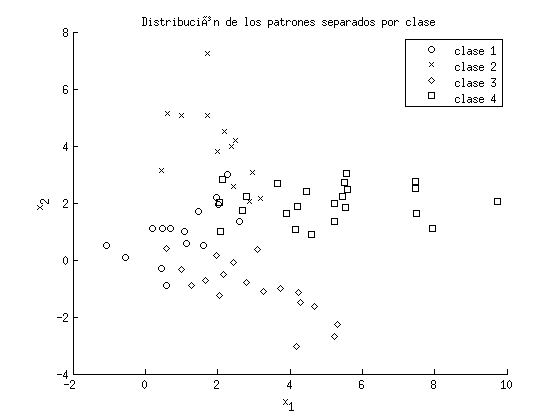
\includegraphics [width=4in]{Ejercicio2_01.png}
\begin{par}
Por la gráfica se deduce que deberán utilizarse gaussianas con media desconocida y covarianza no isotropica desconocida. Separo los patrones para entrenamiento para estimar las medias y matrices de covarianzas de cada clase.
\end{par} \vspace{1em}
\begin{verbatim}
% Divido los patrones a utilizar en el entrenamiento de los de testeo
nentre = floor(0.8 * N); % 80% de los patrones para entrenamiento
ntest = N - nentre;      % 20% de los patrones para testeo
ientre = randperm(N,nentre); % indices utilizados en el entrenamiento
itest = setdiff(1:N,ientre); % indices utilizados para el testeo

% Estimación de los parámetros para cada clase, con los patrones de
% entrenamiento
% medias estimadas
u1 = mean(x(intersect(c1,ientre),:));
u2 = mean(x(intersect(c2,ientre),:));
u3 = mean(x(intersect(c3,ientre),:));
u4 = mean(x(intersect(c4,ientre),:));
% matrices de covarianzas estimadas
sig1 = cov(x(intersect(c1,ientre),:));
sig2 = cov(x(intersect(c2,ientre),:));
sig3 = cov(x(intersect(c3,ientre),:));
sig4 = cov(x(intersect(c4,ientre),:));

% clasifico los patrones de entrenamiento
centre = zeros(size(c)); % clases asignadas durante el entrenamiento
for n = ientre
    xn = x(n,:); % voy leyendo de a un dato

    % Calculo los valores de las funciones discriminantes para xn
    g1 = mvnpdf(xn, u1, sig1);
    g2 = mvnpdf(xn, u2, sig2);
    g3 = mvnpdf(xn, u3, sig3);
    g4 = mvnpdf(xn, u4, sig4);

    % Busco cual es la clase ganadora, asigno 0 si cae en la frontera
    if     g1 > max([g2 g3 g4])
        centre(n) = 1;
    elseif g2 > max([g1 g3 g4])
        centre(n) = 2;
    elseif g3 > max([g1 g2 g4])
        centre(n) = 3;
    elseif g4 > max([g1 g2 g3])
        centre(n) = 4;
    else
        centre(n) = 0;
    end
end

% busco cuales patrones fueron confundidos al clasificar
cmal = intersect(find(c~=centre), ientre); % patrones mal identificados
cbien = setdiff(ientre,cmal); % patrones identificados correctamente

fprintf('La tasa de aciertos en el entrenamiento es de %0.2f %%\n', ...
        100*length(cbien)/nentre);
% disp(['La tasa de aciertos es de ' num2str(100*nnz(cright)/N) '%'])

hold on; plot(x(cmal,1), x(cmal,2), '.r'); hold off
\end{verbatim}

        \color{lightgray} \begin{verbatim}La tasa de aciertos en el entrenamiento es de 87.27 %
\end{verbatim} \color{black}
    
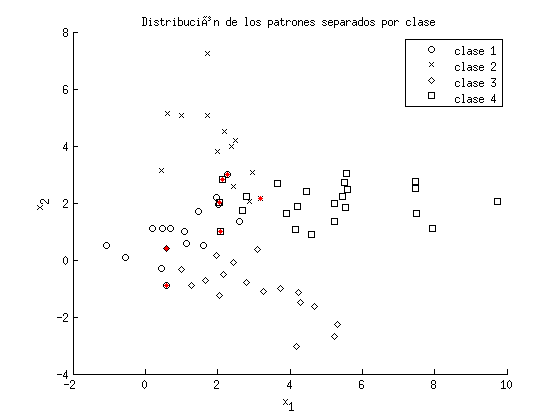
\includegraphics [width=4in]{Ejercicio2_02.png}
\begin{par}
Los patrones de entrenamiento mal clasificados se indican con un punto rojo en la misma gráfica.
\end{par} \vspace{1em}
\begin{par}
Ahora clasifico los patrones de testeo y calculo la tasa de reconocimiento.
\end{par} \vspace{1em}
\begin{verbatim}
% clasifico los patrones de testeo
% --------------------------------
ctest = zeros(size(c)); % clases asignadas durante el testeo
for n = itest
    xn = x(n,:); % voy leyendo de a un dato

    % Calculo los valores de las funciones discriminantes para xn
    g1 = mvnpdf(xn, u1, sig1);
    g2 = mvnpdf(xn, u2, sig2);
    g3 = mvnpdf(xn, u3, sig3);
    g4 = mvnpdf(xn, u4, sig4);

    % Busco cual es la clase ganadora, asigno 0 si cae en la frontera
    if     g1 > max([g2 g3 g4])
        ctest(n) = 1;
    elseif g2 > max([g1 g3 g4])
        ctest(n) = 2;
    elseif g3 > max([g1 g2 g4])
        ctest(n) = 3;
    elseif g4 > max([g1 g2 g3])
        ctest(n) = 4;
    else
        ctest(n) = 0;
    end
end

% busco cuales patrones fueron confundidos al clasificar
cmal = intersect(find(c~=ctest), itest); % patrones mal identificados
cbien = setdiff(itest,cmal); % patrones identificados correctamente

fprintf('La tasa de aciertos en el testeo es de %0.2f %%\n', ...
        100*length(cbien)/ntest);

hold on; plot(x(cmal,1), x(cmal,2), '*b'); hold off
\end{verbatim}

        \color{lightgray} \begin{verbatim}La tasa de aciertos en el testeo es de 78.57 %
\end{verbatim} \color{black}
    
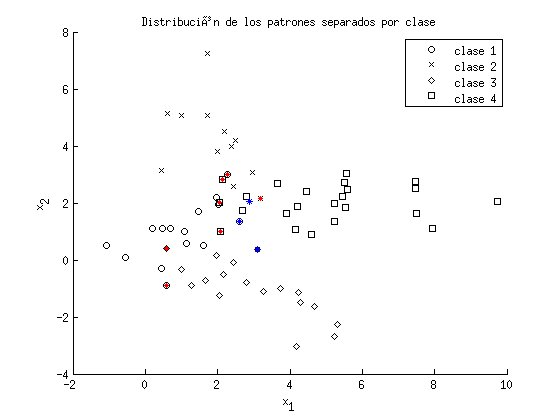
\includegraphics [width=4in]{Ejercicio2_03.png}
\begin{par}
Los patrones de testeo mal clasificados se indican con un asterisco azul en la misma gráfica.
\end{par} \vspace{1em}
\begin{par}
Por último realizo una gráfica representativa de las regiones definidas durante el entrenamiento
\end{par} \vspace{1em}
\begin{verbatim}
T = 100;
x1 = linspace(-2,10,T);
x2 = linspace(-4,8,T);
[X1,X2] = meshgrid(x1,x2);
for i = 1:T
    for j = 1:T
        xn = [x1(i) x2(j)];
        gc1(i,j) = mvnpdf(xn, u1, sig1);
        gc2(i,j) = mvnpdf(xn, u2, sig2);
        gc3(i,j) = mvnpdf(xn, u3, sig3);
        gc4(i,j) = mvnpdf(xn, u4, sig4);
    end
end

gc1234 = cat(3, gc1, gc2, gc3, gc4);

[maxg, maxc] = max(gc1234,[],3);

figure
grises = linspace(0.7,0.9,64);
colormap(repmat(grises',1,3))
surf(X1,X2,maxc'-4,'EdgeColor','none')
hold on; contour(X1,X2,maxg',5,'k'); hold off;
view(2); axis square
xlabel('x_1'); ylabel('x_2');
title('Regiones de decisión')

text([u1(1) u2(1) u3(1) u4(1)], [u1(2) u2(2) u3(2) u4(2)],...
    {'C_1','C_2','C_3','C_4'})
\end{verbatim}

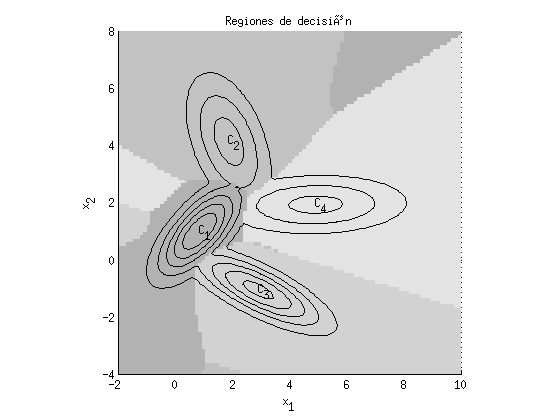
\includegraphics [width=4in]{Ejercicio2_04.png}



\end{document}
    
